%!Mode::"UTF-8"
\documentclass[12pt]{article}

% 页面设置
\usepackage{geometry}
\geometry{left=2.5cm, right=2.5cm, top=2.5cm, bottom=2.5cm}
\usepackage{graphicx}
\usepackage{ctex}
\usepackage{fontspec}
\usepackage{setspace}

% 代码设置
\usepackage{listings}
\usepackage{color}
\setmonofont{Consolas}
\definecolor{listing}{gray}{0.97}
\lstset{
	backgroundcolor=\color{listing},
	basicstyle=\footnotesize,
	numbers=left,
	numberstyle=\footnotesize,
	stepnumber=1,
	aboveskip={0.5\baselineskip},
	belowskip={0.5\baselineskip},
	columns=fullflexible,
	breaklines=true,
	breakatwhitespace=true,
	frame=single,
	basicstyle=\ttfamily,
	numberstyle=\ttfamily,
	tabsize=2
}

% 字体设置
\setmainfont{Times New Roman}
\setCJKmainfont{SimSun}
\setCJKsansfont{SimHei}

% 表格设置
\usepackage{makecell}
\newcommand{\addcell}[2][4]{\makecell{\zihao{#1}\textsf{#2}}}
\usepackage{titlesec}
\usepackage{booktabs}
\usepackage{tabularx}

% 设置图注、表注
\usepackage{caption}
\usepackage{bicaption}
\captionsetup{labelsep=quad, font={small, bf}, skip=2pt}
\DeclareCaptionOption{english}[]{
    \renewcommand\figurename{Fig.}
    \renewcommand\tablename{Table}
}
\captionsetup[bi-second]{english}

% 设置页眉
\usepackage{fancyhdr}
\pagestyle{fancy}
\fancypagestyle{preContent}{
    \fancyhead[L]{\zihao{-5} 物理化学实验}
    \fancyhead[C]{\zihao{-5} 实验三\ \ 液体饱和蒸气压的测定}
    \fancyhead[R]{\zihao{-5} 1800011828\ 王宇哲}
}
\pagestyle{preContent}

%	设置首页页眉页脚
\fancypagestyle{plain}{
	\fancyhead[L]{\zihao{-5} 物理化学实验}
	\fancyhead[C]{\zihao{-5} 实验三\ \ 液体饱和蒸气压的测定}
	\fancyhead[R]{\zihao{-5} 1800011828\ 王宇哲}
	\cfoot{}
}

% 设置标题格式
\titleformat*{\section}{\zihao{4}\sffamily}
\titleformat*{\subsection}{\zihao{-4}\sffamily}
\titleformat*{\subsubsection}{\zihao{-4}\sffamily}
\titlespacing*{\section}{0pt}{10pt}{10pt}
\titlespacing*{\subsection}{0pt}{10pt}{5pt}
\titlespacing*{\subsubsection}{0pt}{10pt}{5pt}

% 设置引用格式
\usepackage[super,round,comma,compress]{natbib}

\usepackage{amsmath}
\usepackage{amssymb}

%设置封面
\begin{document}
    % 标题页
    \begin{titlepage}
    	% 页眉
    	\thispagestyle{plain}
        % 图片
        \begin{figure}[h]
            \centering
            \includegraphics{pku.png}
        \end{figure}
        \vspace{24pt}
        % 标题
        \centerline{\zihao{-0} \textsf{物理化学实验报告}}
        \vspace{40pt} % 空行
        \begin{center}
            \begin{tabular}{cp{8.5 cm}}
                % 题目
                \addcell[2]{题目:\ } & \addcell[2]{液体饱和蒸气压的测定} \\
                \cline{2-2}
            \end{tabular}
        \end{center}
        \vspace{20pt} % 空行
        \begin{center}
            \doublespacing
            \begin{tabular}{cp{5cm}}
                % 姓名
                \addcell{姓\phantom{空格}名:\ } & \addcell{王宇哲} \\
                \cline{2-2}
                % 学号
                \addcell{学\phantom{空格}号:\ } & \addcell{1800011828}\\
                \cline{2-2}
                % 组别
                \addcell{组\phantom{空格}别:\ } & \addcell{11组} \\
                \cline{2-2}
                % 实验日期
                \addcell{实验日期:\ } & \addcell{2020.12.2}\\
                \cline{2-2}
                % 室温
                \addcell{室\phantom{空格}温:\ } & \addcell{291.75\ K}\\
                \cline{2-2}
                % 大气压强
                \addcell{大气压强:\ } & \addcell{103.46\ kPa}\\
                \cline{2-2}
            \end{tabular}
            \begin{tabular*}{\textwidth}{c}
                \\ % 这是空行
                \\ % 这是空行
                \\ % 这是空行
                \\ % 这是空行
                \hline % 分割线
            \end{tabular*}
        \end{center}
        % 摘要
        \textsf{摘\ \ 要}\ \ 本实验使用静态法测$\rm CCl_{4}$不同温度的饱和蒸气压,测得$\rm CCl_{4}$常压沸点$T_{b}=(350.17\pm 0.01)\ \ {\rm K}$,平均摩尔气化热$\Delta^{\rm g}_{\rm l}H_{m}=(30.87\pm 0.02)\ \ {\rm kJ\cdot mol^{-1}}$,摩尔气化熵$\Delta^{\rm g}_{\rm l}S_{m}=(88.16\pm 0.06)\ \ {\rm J\cdot K^{-1}\cdot mol^{-1}}$。使用动态法测$\rm H_{2}O$不同温度的饱和蒸气压,测得$\rm H_{2}O$常压沸点$T_{b}=(373.50\pm 0.01)\ \ {\rm K}$,平均摩尔气化热$\Delta^{\rm g}_{\rm l}H_{m}=(41.01\pm 0.08)\ \ {\rm kJ\cdot mol^{-1}}$,摩尔气化熵$\Delta^{\rm g}_{\rm l}S_{m}=(109.8\pm 0.2)\ \ {\rm J\cdot K^{-1}\cdot mol^{-1}}$。验证了$\rm CCl_{4}$的摩尔气化熵大致符合褚鲁统规则预测,而$\rm H_{2}O$不符合褚鲁统规则。
        \\
        \\
        % 关键字
        \textsf{关键词}\ \ 饱和蒸气压;摩尔气化热;Clausius-Clapeyron方程;褚鲁统规则
    \end{titlepage}

    \section{引言}
	略
               
\vbox{}        
    \section{实验部分}
    	\subsection{仪器和试剂}
    	$\rm CCl_{4}$,二次去离子水,$1000\ \ {\rm mL}$烧杯,$250\ \ {\rm mL}$两口圆底烧瓶等。\par 
    	$\rm WXI-04$型压力-温度测定仪,$\rm SHB-III$型循环水泵,电加热器,带电热套的磁力搅拌装置,冷凝水循环系统,真空缓冲罐,直形冷凝管,搅拌磁子,真空脂。
     
\vbox{}
    	 \subsection{实验内容\citealp{physchemlab}}
			\subsubsection{静态法测$\rm CCl_{4}$饱和蒸气压}
实验开始前,读取实验室内的大气压$p_{0}=103.48\ \ {\rm kPa}$,温度$t=18.6\ \ {\rm ^{\circ}C}$。\par
利用前一组同学已验证气密性的测量系统直接进行实验,压力计的零点为$p_{1}=-0.57\ \ {\rm kPa}$。测$\rm CCl_{4}$大气压下的沸点。使体系与大气相通,水浴加热至$\sim 80\ \ {\rm ^{\circ}C}$,平衡管中有气泡产生,将平衡管中的空气排净。停止加热,不断搅拌,温度下降至一定程度时,$b$管中气泡开始消失,$c$管液面开始上升,同时$b$管液面下降。两管液面达到同一水平时,立即记下此时的温度计示数$t_{b}$和压力计示数$p^{\prime}$,重复赶气,平行测量多次$\rm CCl_{4}$大气压下的沸点,直至结果一致。\par 
立即关闭储气罐通向大气的活塞,先打开真空泵,再打开通真空泵的阀,使体系减压$\sim 5\ \ {\rm kPa}$,液体重又沸腾。关闭通真空泵的阀,不断搅拌,冷却至$b$、$c$两管液面等高时,按下温度-压力测定仪上的绿色按钮,记录温度$t_{b}$和压力计示数$p^{\prime}$。继续实验,每次减压$\sim 5\ \ {\rm kPa}$,直至压差值为$\sim 50\ \ {\rm kPa}$时,停止实验。

\subsubsection{动态法测$\rm H_{2}O$饱和蒸气压}
组装测量系统。将装有约$200\ \ {\rm mL}$去离子水和搅拌磁子的两口圆底烧瓶置于电加热套上并与冷凝管相连接。将温度探头通过橡皮塞插入烧瓶的侧口,探头尖端位于液面上侧,磨口处涂抹真空脂以防止漏气。打开回流冷凝水,调节流量适中。旋转储气罐阀门使系统与大气相通,读取压力计的零点为$p_{2}=-0.59\ \ {\rm kPa}$。打开公用循环真空泵,旋转储气罐阀门,使系统与大气隔绝、与真空泵相通,使压力计示数降至$-53.18\ \ {\rm kPa}$;关闭活塞使系统与真空泵隔绝,$3\ \ {\rm min}$后压力计示数为$-53.15\ \ {\rm kPa}$,表明体系气密性符合要求。\par
保持压差值为$\sim 50\ \ {\rm kPa}$,开始加热,不断搅拌。记录烧瓶中水沸腾、温度计示数不再上升时的温度$t_{b}$和压力计示数$p^{\prime}$。停止加热,略微开启缓冲罐通大气的阀门,使少量空气进入系统,使内外压差降低$\sim 5\ \ {\rm kPa}$,关闭活塞,重新加热至沸腾,记录$t_{b}$和$p^{\prime}$。重复上述步骤,直至系统与大气完全相通。继续加热,测量$\rm H_{2}O$大气压下的沸点。平行测量3次,每次等体系温度略微冷却、水不再沸腾后重新加热至沸腾后测量。\par 
实验结束后,读取实验室内的大气压$p_{0}=103.43\ \ {\rm kPa}$,取实验前后大气压的平均值$p_{0}=103.46\ \ {\rm kPa}$作为实验过程中的大气压值。   			

\vbox{}
 \section{数据与结果}
 \subsection{实验数据记录及处理}
 \subsubsection{静态法测$\rm CCl_{4}$饱和蒸气压}
使用静态法测定$\rm CCl_{4}$大气压下的沸点,平行测量4组数据;考虑到压力计的零点$p_{1}=-0.57\ \ {\rm kPa}$,对测量得到的内外压强差$p^{\prime}$进行零点修正,得到实际的内外压强差$p_{1}^{\prime}=p^{\prime}-p_{1}$;根据实验过程中的大气压$p_{0}=103.46\ \ {\rm kPa}$,计算$\rm CCl_{4}$的饱和蒸气压$ p=p^{\prime}_{1}+p_{0}$,结果如\textbf{表1}所示。
 \begin{table}[h]
 	\centering
 	\zihao{5}
 	\bicaption{$\rm CCl_{4}$常压沸点测定实验数据}{$\rm CCl_{4}$ Boiling Point Measurement Data at Normal Pressure}
 	\begin{tabular}{ccccc}
 		\toprule
 		编号 & $t_{b}/{\rm ^{\circ}C}$& $p^{\prime}/{\rm kPa}$ & $p_{1}^{\prime}/{\rm kPa}$ & $p/{\rm kPa}$  \\
 		\midrule
 		1 & 76.87 & -0.59 & -0.02 & 103.44 \\
 		2 & 77.01 & -0.60 & -0.03 & 103.43 \\
 		3 & 77.03 & -0.62 & -0.05 & 103.41 \\
 		4 & 77.03 & -0.60 & -0.03 & 103.43 \\
 		\bottomrule
 	\end{tabular}
 \end{table}
 \par
根据\textbf{表1}数据,第1组实验测得$\rm CCl_{4}$常压沸点$t_{b}$与其他3组有较大差别,推测可能原因是在进行第1组实验时平衡管$c$管内空气尚未赶净,$\rm CCl_{4}$分压小于实际压强,导致测得$\rm CCl_{4}$常压沸点偏低。第$2\sim 4$组实验测得常压沸点$t_{b}$结果基本一致,说明平衡管中空气已经排净。计算$\rm CCl_{4}$常压沸点的平均值
$$
t_{b}=\frac{77.01+77.03+77.03}{3} \ \ {\rm ^{\circ}C}=77.02\ \ {\rm {^{\circ}C}}
$$
常压沸点$t_{b}$的不确定度
$$
\sigma_{t_{b}}=\sqrt{\frac{0.01^{2}\times 3}{3-1}} \ \ {\rm K}=0.01\ \ {\rm K} 
$$
故测得$\rm CCl_{4}$常压沸点(换算成热力学温标)为
$$
T_{b}=(350.17\pm 0.01)\ \ {\rm K}
$$
\par
使用静态法测定不同压力下$\rm CCl_{4}$的沸点$t_{b}$;类似地,考虑到压力计的零点$p_{1}=-0.57\ \ {\rm kPa}$,对测量得到的内外压强差$p^{\prime}$进行零点修正,得到实际的内外压强差$p_{1}^{\prime}=p^{\prime}-p_{1}$;根据实验过程中的大气压$p_{0}=103.46\ \ {\rm kPa}$,计算$\rm CCl_{4}$的饱和蒸气压$ p=p^{\prime}_{1}+p_{0}$,结果如\textbf{表2}所示。
 \begin{table}[h]
	\centering
	\zihao{5}
	\bicaption{静态法测$\rm CCl_{4}$沸点实验数据}{$\rm CCl_{4}$ Boiling Point Measurement Data by Static Method}
	\begin{tabular}{ccccc}
		\toprule
		编号 & $t_{b}/{\rm ^{\circ}C}$& $p^{\prime}/{\rm kPa}$ & $p_{1}^{\prime}/{\rm kPa}$ & $p/{\rm kPa}$  \\
		\midrule
		1  & 75.56 & -4.86  & -4.29  & 99.17 \\
		2  & 73.69 & -10.48 & -9.91  & 93.55 \\
		3  & 71.94 & -15.40 & -14.83 & 88.63 \\
		4  & 70.14 & -20.24 & -19.67 & 83.79 \\
		5  & 67.63 & -26.61 & -26.04 & 77.42 \\
		6  & 66.25 & -30.01 & -29.44 & 74.02 \\
		7  & 64.08 & -35.03 & -34.46 & 69.00 \\
		8  & 61.80 & -40.00 & -39.43 & 64.03 \\
		9  & 59.24 & -45.27 & -44.70 & 58.76 \\
		10 & 56.54 & -50.41 & -49.84 & 53.62 \\
		\bottomrule
	\end{tabular}
\end{table}
\par

 
\subsubsection{动态法测$\rm H_{2}O$饱和蒸气压}
使用动态法测定不同压力下$\rm H_{2}O$的沸点$t_{b}$;考虑到压力计的零点$p_{2}=-0.59\ \ {\rm kPa}$,对测量得到的内外压强差$p^{\prime}$进行零点修正,得到实际的内外压强差$p_{2}^{\prime}=p^{\prime}-p_{2}$;根据实验过程中的大气压$p_{0}=103.46\ \ {\rm kPa}$,计算$\rm CCl_{4}$的饱和蒸气压$ p=p^{\prime}_{2}+p_{0}$,结果如\textbf{表3}所示。
 \begin{table}[h]
	\centering
	\zihao{5}
	\bicaption{动态法测$\rm H_{2}O$沸点实验数据}{$\rm H_{2}O$ Boiling Point Measurement Data by Dynamic Method}
	\begin{tabular}{ccccc}
		\toprule
		编号 & $t_{b}/{\rm ^{\circ}C}$& $p^{\prime}/{\rm kPa}$ & $p_{2}^{\prime}/{\rm kPa}$ & $p/{\rm kPa}$  \\
		\midrule
		1  & 81.79 & -52.04 & -51.45 & 52.01  \\
		2  & 84.29 & -46.95 & -46.36 & 57.10  \\
		3  & 86.34 & -42.15 & -41.56 & 61.90  \\
		4  & 88.40 & -37.09 & -36.50 & 66.96  \\
		5  & 90.35 & -32.17 & -31.58 & 71.88  \\
		6  & 92.17 & -27.09 & -26.50 & 76.96  \\
		7  & 93.86 & -22.16 & -21.57 & 81.89  \\
		8  & 95.49 & -17.10 & -16.51 & 86.95  \\
		9  & 96.99 & -12.18 & -11.59 & 91.87  \\
		10 & 98.53 & -7.01  & -6.42  & 97.04  \\
		11 & 99.91 & -1.92  & -1.33  & 102.13 \\
		\bottomrule
	\end{tabular}
\end{table}
\par

使用动态法测定$\rm H_{2}O$大气压下的沸点,平行测量3组数据;类似地,考虑到压力计的零点$p_{2}=-0.59\ \ {\rm kPa}$,对测量得到的内外压强差$p^{\prime}$进行零点修正,得到实际的内外压强差$p_{2}^{\prime}=p^{\prime}-p_{2}$;根据实验过程中的大气压$p_{0}=103.46\ \ {\rm kPa}$,计算$\rm H_{2}O$的饱和蒸气压$ p=p^{\prime}_{2}+p_{0}$,结果如\textbf{表4}所示。
 \begin{table}[h]
	\centering
	\zihao{5}
	\bicaption{$\rm H_{2}O$常压沸点测定实验数据}{$\rm H_{2}O$ Boiling Point Measurement Data at Normal Pressure}
	\begin{tabular}{ccccc}
		\toprule
		编号 & $t_{b}/{\rm ^{\circ}C}$& $p^{\prime}/{\rm kPa}$ & $p_{2}^{\prime}/{\rm kPa}$ & $p/{\rm kPa}$  \\
		\midrule
		1 & 100.34 & -0.42 & 0.17 & 103.63 \\
		2 & 100.36 & -0.40 & 0.19 & 103.65 \\
		3 & 100.36 & -0.39 & 0.20 & 103.66 \\
		\bottomrule
	\end{tabular}
\end{table}
\par
计算$\rm H_{2}O$常压沸点的平均值
$$
t_{b}=\frac{100.34+100.36+100.36}{3} \ \ {\rm ^{\circ}C}=100.35\ \ {\rm {^{\circ}C}}
$$
常压沸点$t_{b}$的不确定度
$$
\sigma_{t_{b}}=\sqrt{\frac{0.01^{2}\times 3}{3-1}} \ \ {\rm K}=0.01\ \ {\rm K} 
$$
故测得$\rm H_{2}O$常压沸点(换算成热力学温标)为
$$
T_{b}=(373.50\pm 0.01)\ \ {\rm K}
$$
\vbox{}
 \subsection{数据处理结果与分析}
 \subsubsection{$\rm CCl_{4}$饱和蒸气压$p$-温度$T$关系与热力学数据计算}
利用$T=t_{b}+273.15\ \ {\rm K}$将$\rm CCl_{4}$的沸点$t_{b}$转化为热力学温标$T$,取标准大气压$p^{\ominus}=100.0\ \ {\rm kPa}$,计算${\rm lg}(p/p^{\ominus})$和$T^{-1}$,结果如\textbf{表5}所示。
\begin{table}[h]
	\centering
	\zihao{5}
	\bicaption{$\rm CCl_{4}$ $p-T$关系相关计算数据}{$\rm CCl_{4}$ $p-T$ Relationship Calculation Data}
	\begin{tabular}{cccccc}
		\toprule
		编号 & $t_{b}/{\rm ^{\circ}C}$& $T/{\rm K}$ & $p/{\rm kPa}$ & ${\rm lg}(p/p^{\ominus})$ & $T^{-1}/{\rm 10^{-3}\ \  K^{-1}}$\\
		\midrule
		1  & 75.56 & 348.71 & 99.17 & -0.003620 & 2.8677 \\
		2  & 73.69 & 346.84 & 93.55 & -0.02896 & 2.8832 \\
		3  & 71.94 & 345.09 & 88.63 & -0.05242 & 2.8978 \\
		4  & 70.14 & 343.29 & 83.79 & -0.07681 & 2.9130 \\
		5  & 67.63 & 340.78 & 77.42 & -0.11115 & 2.9344 \\
		6  & 66.25 & 339.40 & 74.02 & -0.13065 & 2.9464 \\
		7  & 64.08 & 337.23 & 69.00 & -0.16115 & 2.9653 \\
		8  & 61.80 & 334.95 & 64.03 & -0.19362 & 2.9855 \\
		9  & 59.24 & 332.39 & 58.76 & -0.23092 & 3.0085 \\
		10 & 56.54 & 329.69 & 53.62 & -0.27067 & 3.0332 \\
		\bottomrule
	\end{tabular}
\end{table}
\par

根据\textbf{表5}数据,作出$p-T$关系的散点图,并用python SciPy interpolate用曲线平滑连接各散点,作出$p-T$曲线,如\textbf{图1}所示。
\begin{figure}[h]
	\centering
	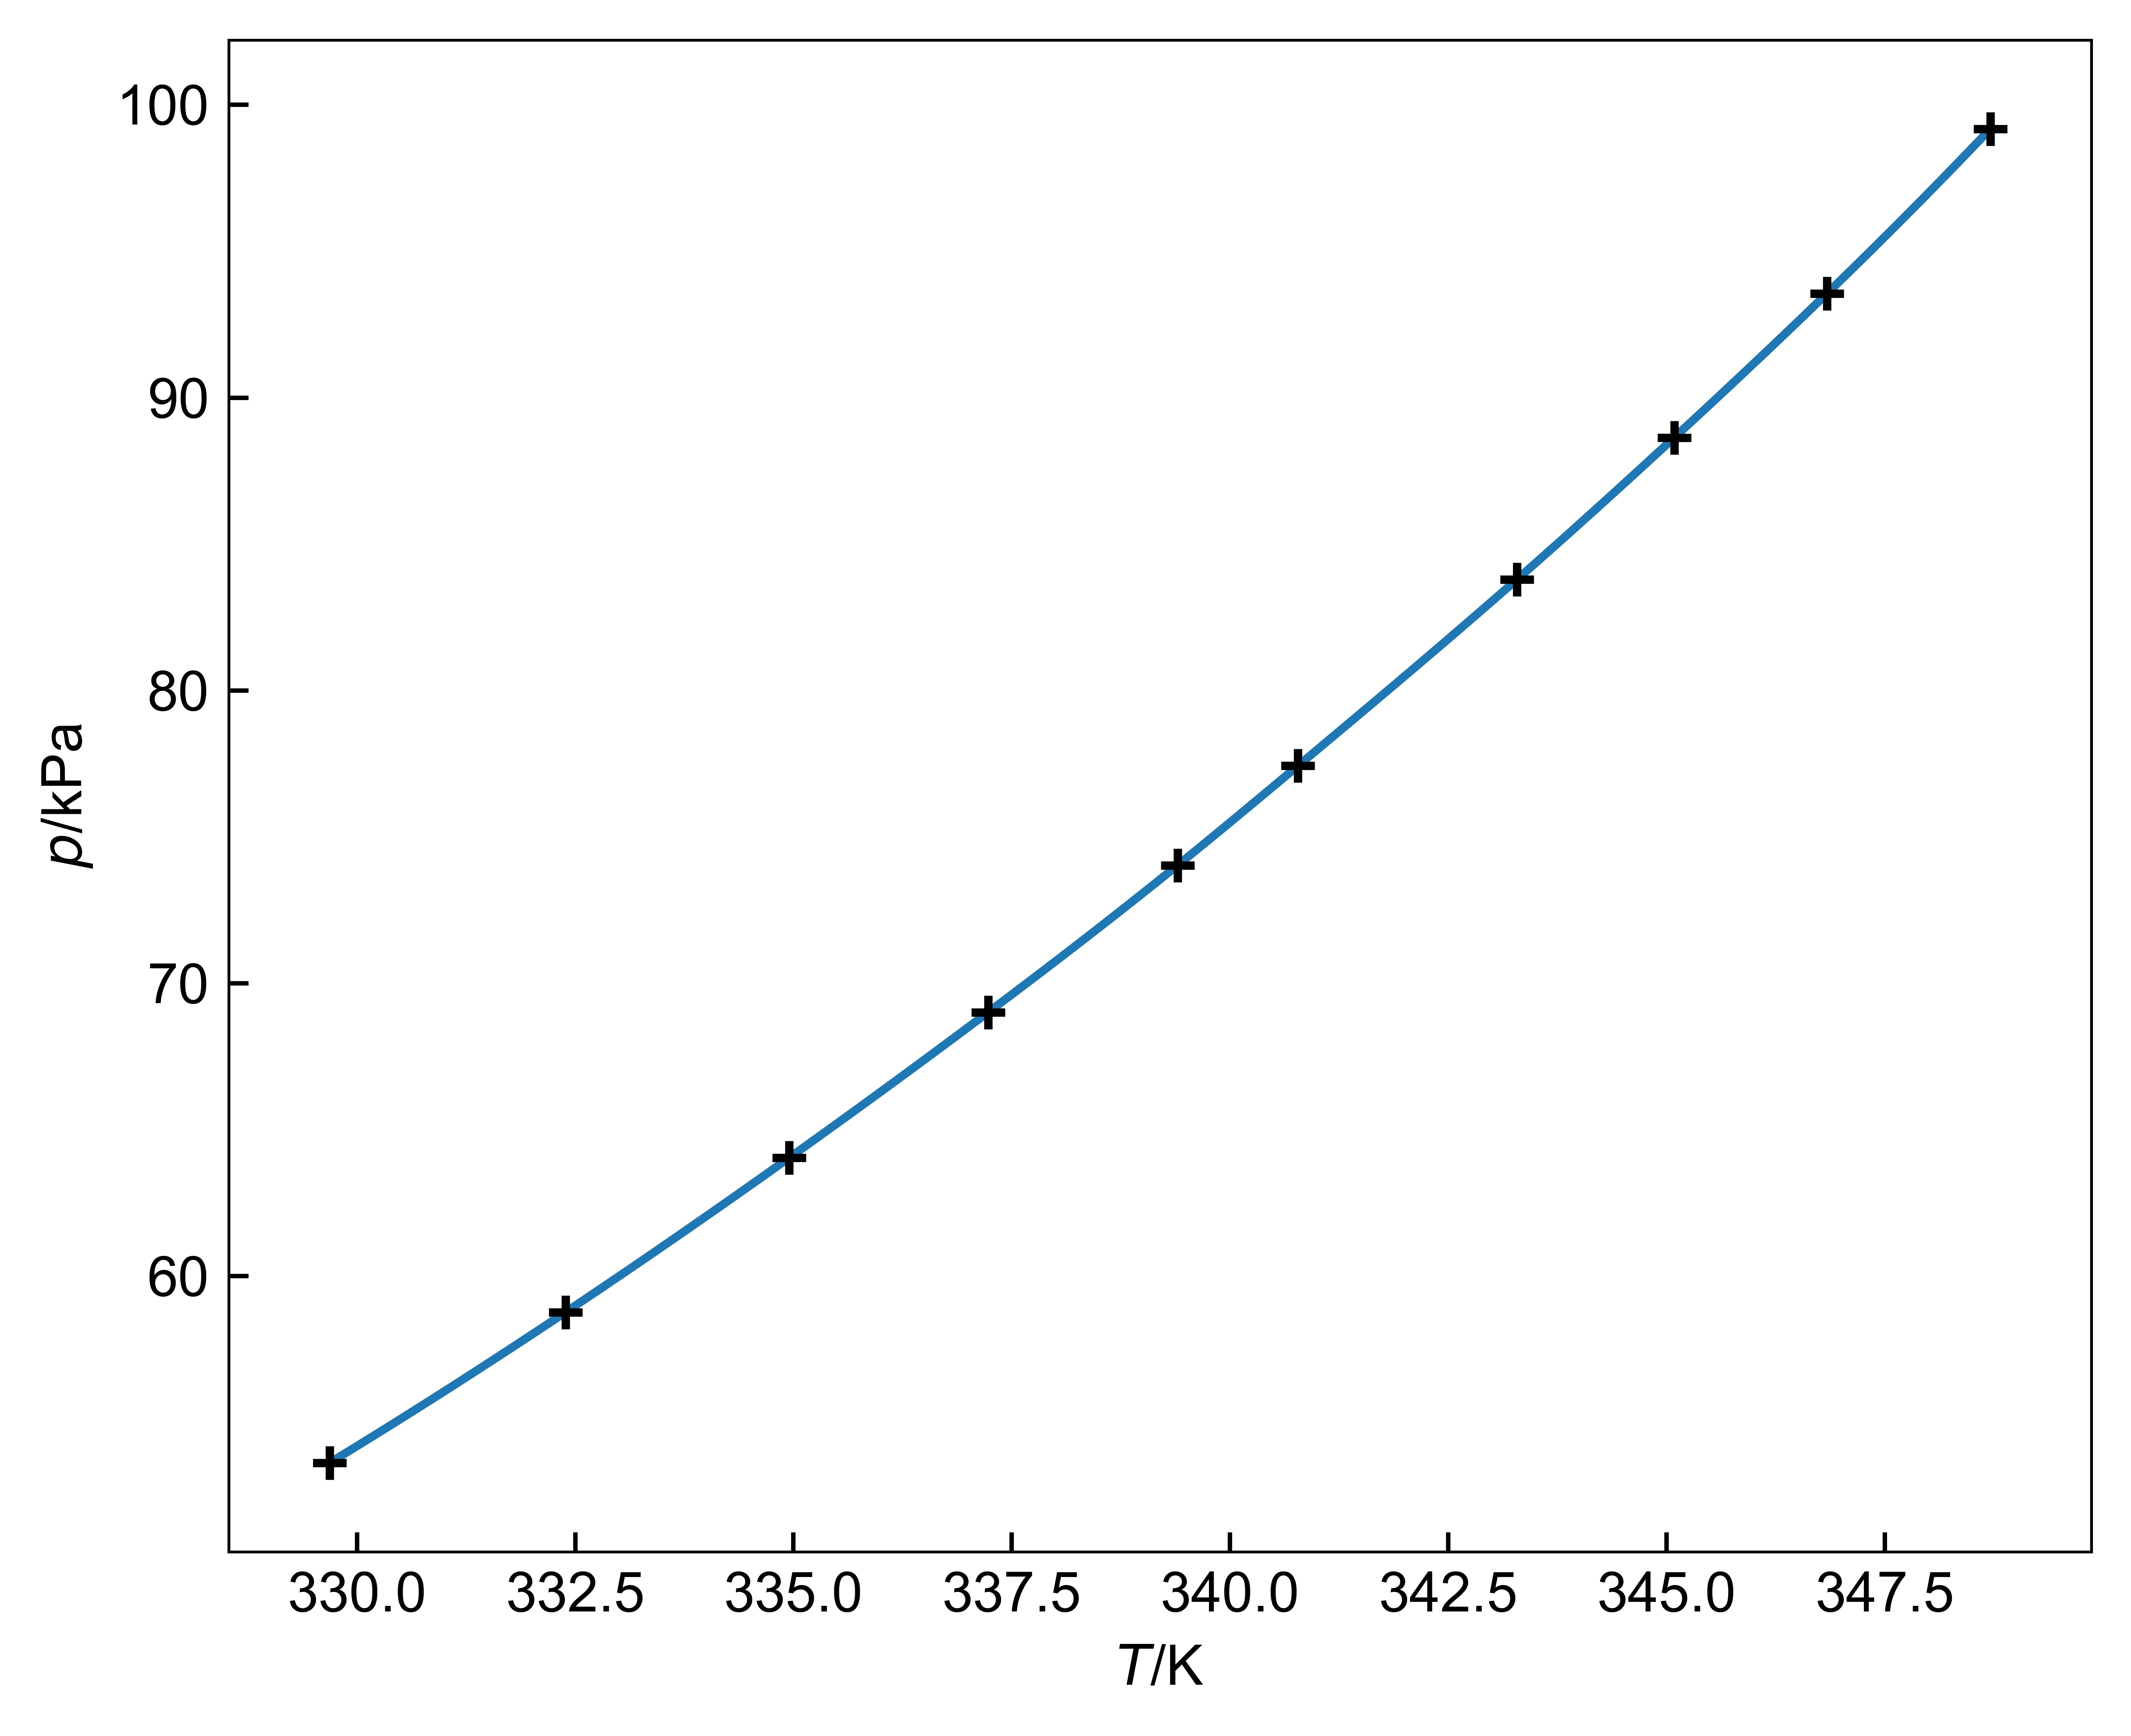
\includegraphics[width=0.6\textwidth]{1.jpg}
	\bicaption{$\rm CCl_{4}$饱和蒸气压$p$-温度$T$曲线}{$p-T$ Diagram of $\rm CCl_{4}$}
\end{figure}
\par
根据Clausius-Clapeyron方程,饱和蒸气压$p$与气液平衡温度$T$之间满足
$$
{\rm lg}\frac{p}{p^{\ominus}}=-\frac{A}{T}+B
$$
其中斜率大小
$$
A=\frac{\Delta^{\rm g}_{\rm l}H_{m}}{2.303R}
$$
根据\textbf{表5}数据,作出${\rm lg}(p/p^{\ominus})$-$T^{-1}$关系的散点图,并用python SciPy lingress进行线性拟合,作出拟合直线,如\textbf{图2}所示。
\begin{figure}[h]
	\centering
	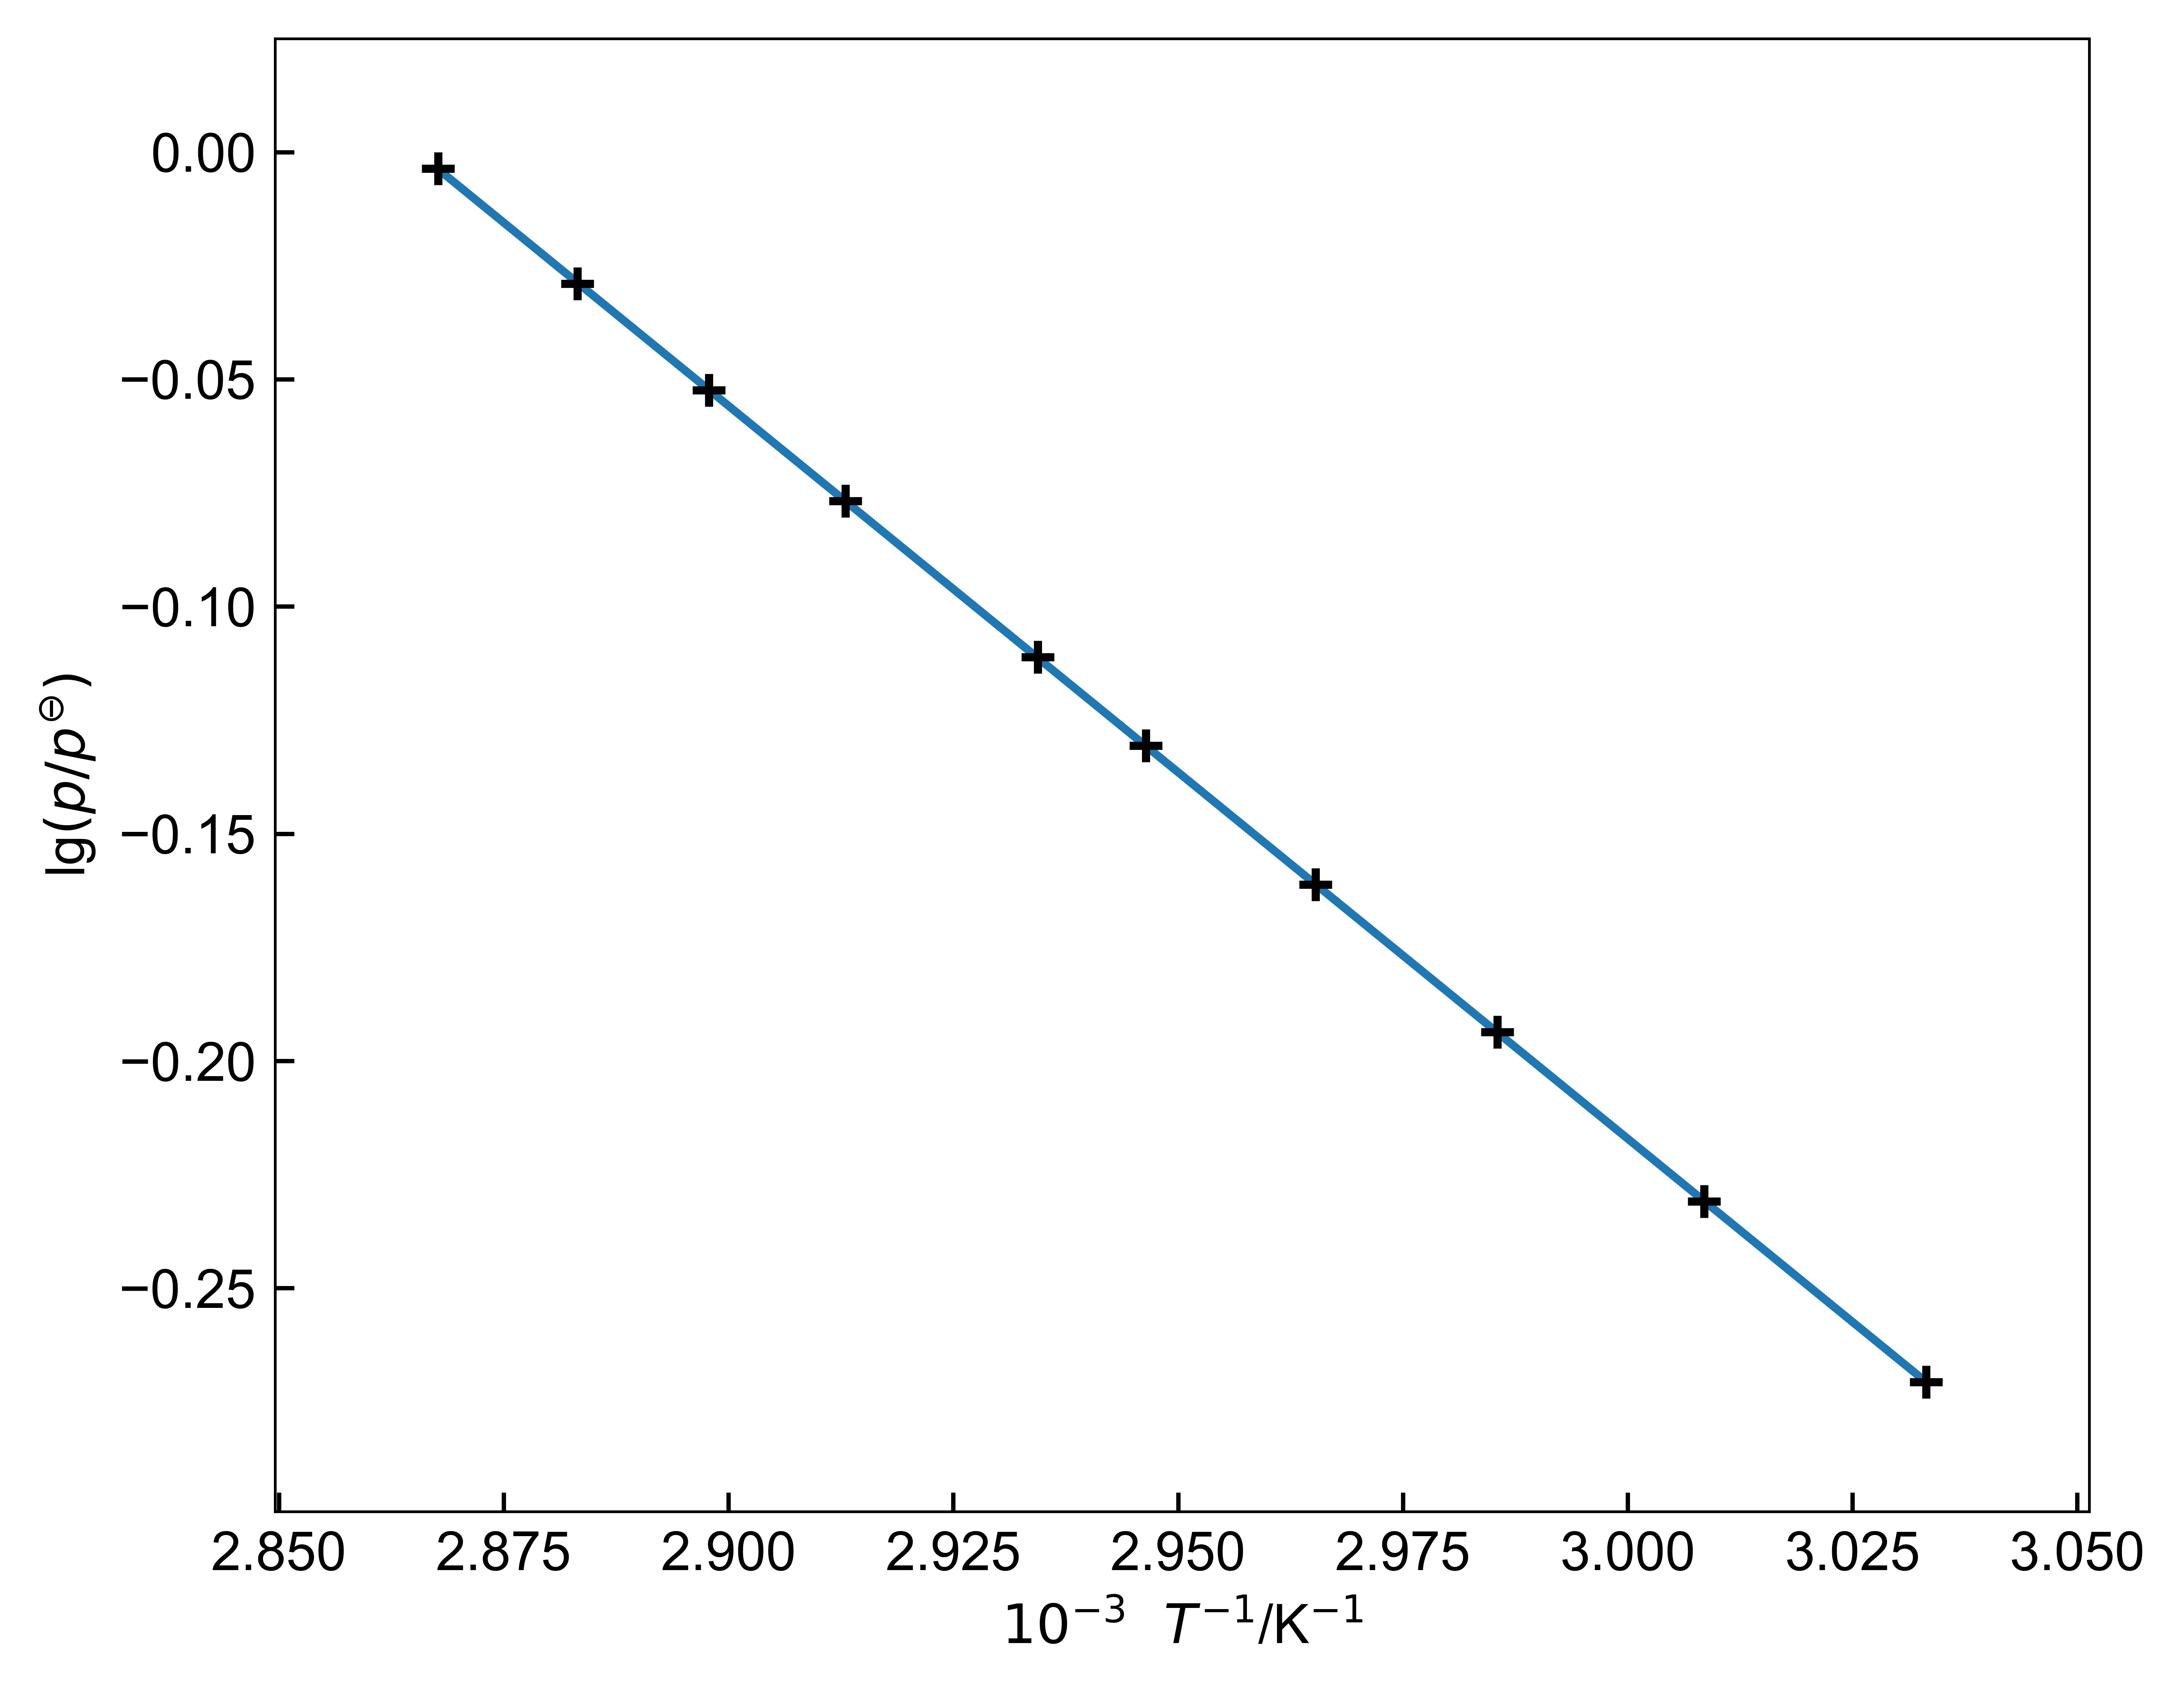
\includegraphics[width=0.6\textwidth]{2.jpg}
	\bicaption{$\rm CCl_{4} \ \ $ ${\rm lg}(p/p^{\ominus})$-$T^{-1}$拟合直线}{${\rm lg}(p/p^{\ominus})$-$T^{-1}$ Fitted Curve of $\rm CCl_{4}$}
\end{figure}
\par
拟合直线的方程为
$$
{\rm lg}(p/p^{\ominus})=-(1.6126\pm 0.0008)\times 10^{3} \ \ T^{-1}/{\rm K^{-1}}+(4.621\pm 0.002),\   \  R=-0.9999991
$$
$|R|\approx 1$,可见${\rm lg}(p/p^{\ominus})$-$T^{-1}$具有很好的线性关系,与Clausius-Clapeyron方程相符。\par 
根据\textbf{图2}中${\rm lg}(p/p^{\ominus})$-$T^{-1}$拟合直线的方程,代入$p=1\ \ {\rm atm}=101.3\ \ {\rm kPa}$,计算$\rm CCl_{4}$的沸点
$$
T=(349.4\pm 0.2)\ \ {\rm K}=(76.2\pm 0.2)\ \ {\rm ^{\circ}C}  
$$
查阅\textit{CRC Handbook of Chemistry and Physics}\citealp{crc},知$\rm CCl_{4}$在$\rm 1\ \ atm$下的沸点$t_{b}=76.7\ \ {\rm ^{\circ}C}$,实验计算结果与参考值相近。\par 
计算$\rm CCl_{4}$的平均摩尔气化热$\Delta^{\rm g}_{\rm l}H_{m}$。根据拟合直线斜率大小
$$
A=\frac{\Delta^{\rm g}_{\rm l}H_{m}}{2.303R}
$$
计算
$$
\Delta^{\rm g}_{\rm l}H_{m}=-2.303RA=30.87\ \ {\rm kJ\cdot mol^{-1}}
$$
$\Delta^{\rm g}_{\rm l}H_{m}$的不确定度
$$
\sigma_{\Delta^{\rm g}_{\rm l}H_{m}}=2.303R\sigma_{A}=0.02\ \ {\rm kJ\cdot mol^{-1}}
$$
故$\rm CCl_{4}$的平均摩尔气化热
$$
\Delta^{\rm g}_{\rm l}H_{m}=(30.87\pm 0.02)\ \ {\rm kJ\cdot mol^{-1}}
$$
查阅\textit{CRC Handbook of Chemistry and Physics}\citealp{crc},知$\rm CCl_{4}$在常压沸点下$\Delta^{\rm g}_{\rm l}H_{m}=29.82\ \ {\rm kJ\cdot mol^{-1}}$,实验计算结果与参考值相近。
\par
计算$\rm CCl_{4}$的摩尔气化熵$\Delta^{\rm g}_{\rm l}S_{m}$。
根据3.1.1,实验测得$\rm CCl_{4}$常压沸点
$$
T_{b}=(350.17\pm 0.01)\ \ {\rm K}
$$
在常压沸点$t_{b}$下,自由能变$\Delta^{\rm g}_{\rm l}G_{m}=0$,故
$$
\Delta^{\rm g}_{\rm l}S_{m}=\frac{\Delta^{\rm g}_{\rm l}H_{m}}{T_{b}}=\frac{30.87\ \ {\rm kJ\cdot mol^{-1}}}{350.17\ \ {\rm K}}=88.16\ \ {\rm J\cdot K^{-1} \cdot mol^{-1}}
$$
$\Delta^{\rm g}_{\rm l}S_{m}$的不确定度
$$
\sigma_{\Delta^{\rm g}_{\rm l}S_{m}}=\frac{1}{T_{b}} \sqrt{\sigma^{2}_{\Delta^{\rm g}_{\rm l}H_{m}}+\frac{\Delta^{\rm g}_{\rm l}H_{m}^{2}}{T_{b}^{2}}\sigma^{2}_{t_{b}}}=0.06\ \ {\rm J\cdot K^{-1}\cdot mol^{-1}}
$$
故$\rm CCl_{4}$的摩尔气化熵
$$
\Delta^{\rm g}_{\rm l}S_{m}=(88.16\pm 0.06)\ \ {\rm J\cdot K^{-1} \cdot mol^{-1}}
$$
根据褚鲁统规则,在常压沸点下各正常液体的摩尔熵相同,为$\Delta S\approx 88\ \ {\rm J\cdot K^{-1}\cdot mol^{-1}}$。实验得到$\rm CCl_{4}$摩尔气化熵的计算结果与褚鲁统规则很好地相符。

\subsubsection{$\rm H_{2}O$饱和蒸气压$p$-温度$T$关系与热力学数据计算}
利用$T=t_{b}+273.15\ \ {\rm K}$将$\rm H_{2}O$的沸点$t_{b}$转化为热力学温标$T$,取标准大气压$p^{\ominus}=100.0\ \ {\rm kPa}$,计算${\rm lg}(p/p^{\ominus})$和$T^{-1}$,结果如\textbf{表6}所示。
\begin{table}[h]
	\centering
	\zihao{5}
	\bicaption{$\rm H_{2}O$ $p-T$关系相关计算数据}{$\rm H_{2}O$ $p-T$ Relationship Calculation Data}
	\begin{tabular}{cccccc}
		\toprule
		编号 & $t_{b}/{\rm ^{\circ}C}$& $T/{\rm K}$ & $p/{\rm kPa}$ & ${\rm lg}(p/p^{\ominus})$ & $T^{-1}/{\rm 10^{-3}\ \ K^{-1}}$\\
		\midrule
		1  & 81.79 & 354.94 & 52.01  & -0.28391 & 2.8174 \\
		2  & 84.29 & 357.44 & 57.10  & -0.24336 & 2.7977 \\
		3  & 86.34 & 359.49 & 61.90  & -0.20831 & 2.7817 \\
		4  & 88.40 & 361.55 & 66.96  & -0.17418 & 2.7659 \\
		5  & 90.35 & 363.50 & 71.88  & -0.14339 & 2.7510 \\
		6  & 92.17 & 365.32 & 76.96  & -0.11373 & 2.7373 \\
		7  & 93.86 & 367.01 & 81.89  & -0.08677 & 2.7247 \\
		8  & 95.49 & 368.64 & 86.95  & -0.06073 & 2.7127 \\
		9  & 96.99 & 370.14 & 91.87  & -0.03683 & 2.7017 \\
		10 & 98.53 & 371.68 & 97.04  & -0.01305 & 2.6905 \\
		11 & 99.91 & 373.06 & 102.13 & 0.009153 & 2.6805 \\
		\bottomrule
	\end{tabular}
\end{table}
\par

根据\textbf{表6}数据,作出$p-T$关系的散点图,并用python SciPy interpolate用曲线平滑连接各散点,作出$p-T$曲线,如\textbf{图3}所示。
\begin{figure}[h]
	\centering
	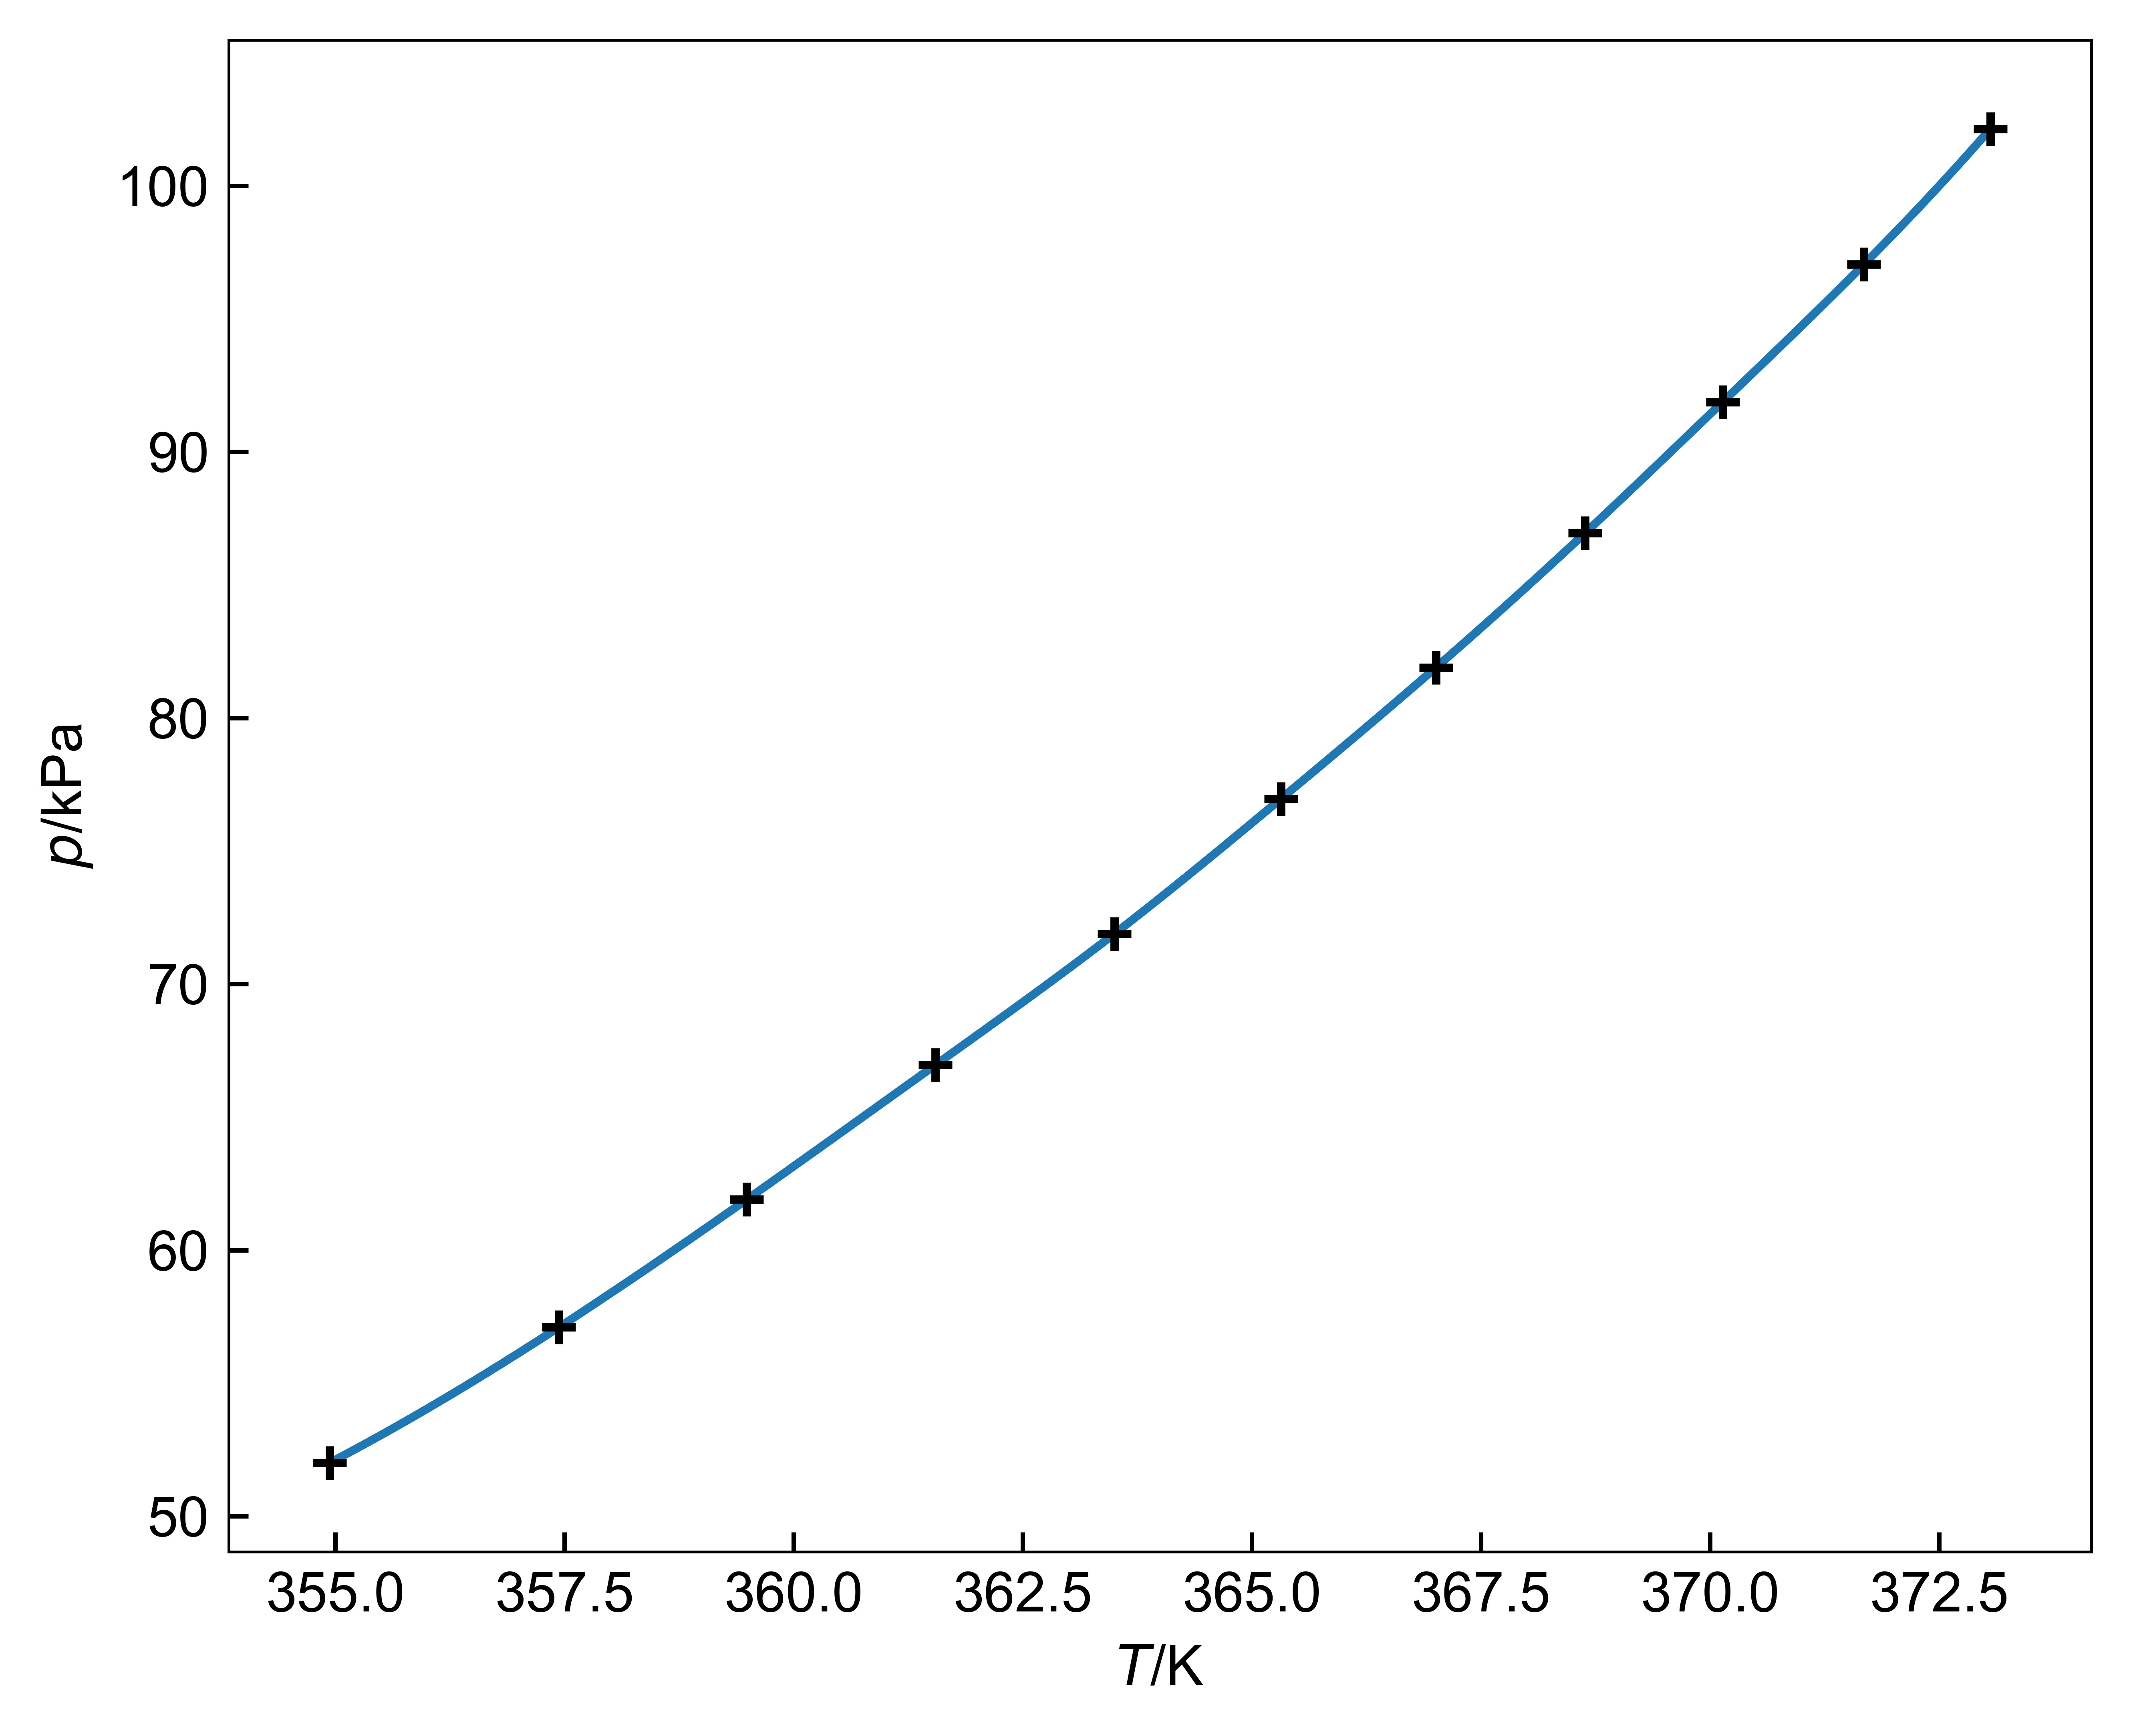
\includegraphics[width=0.6\textwidth]{3.jpg}
	\bicaption{$\rm H_{2}O$饱和蒸气压$p$-温度$T$曲线}{$p-T$ Diagram of $\rm H_{2}O$}
\end{figure}
\par

根据\textbf{表6}数据,作出${\rm lg}(p/p^{\ominus})$-$T^{-1}$关系的散点图,并用python SciPy lingress进行线性拟合,作出拟合直线,如\textbf{图4}所示。
\begin{figure}[h]
	\centering
	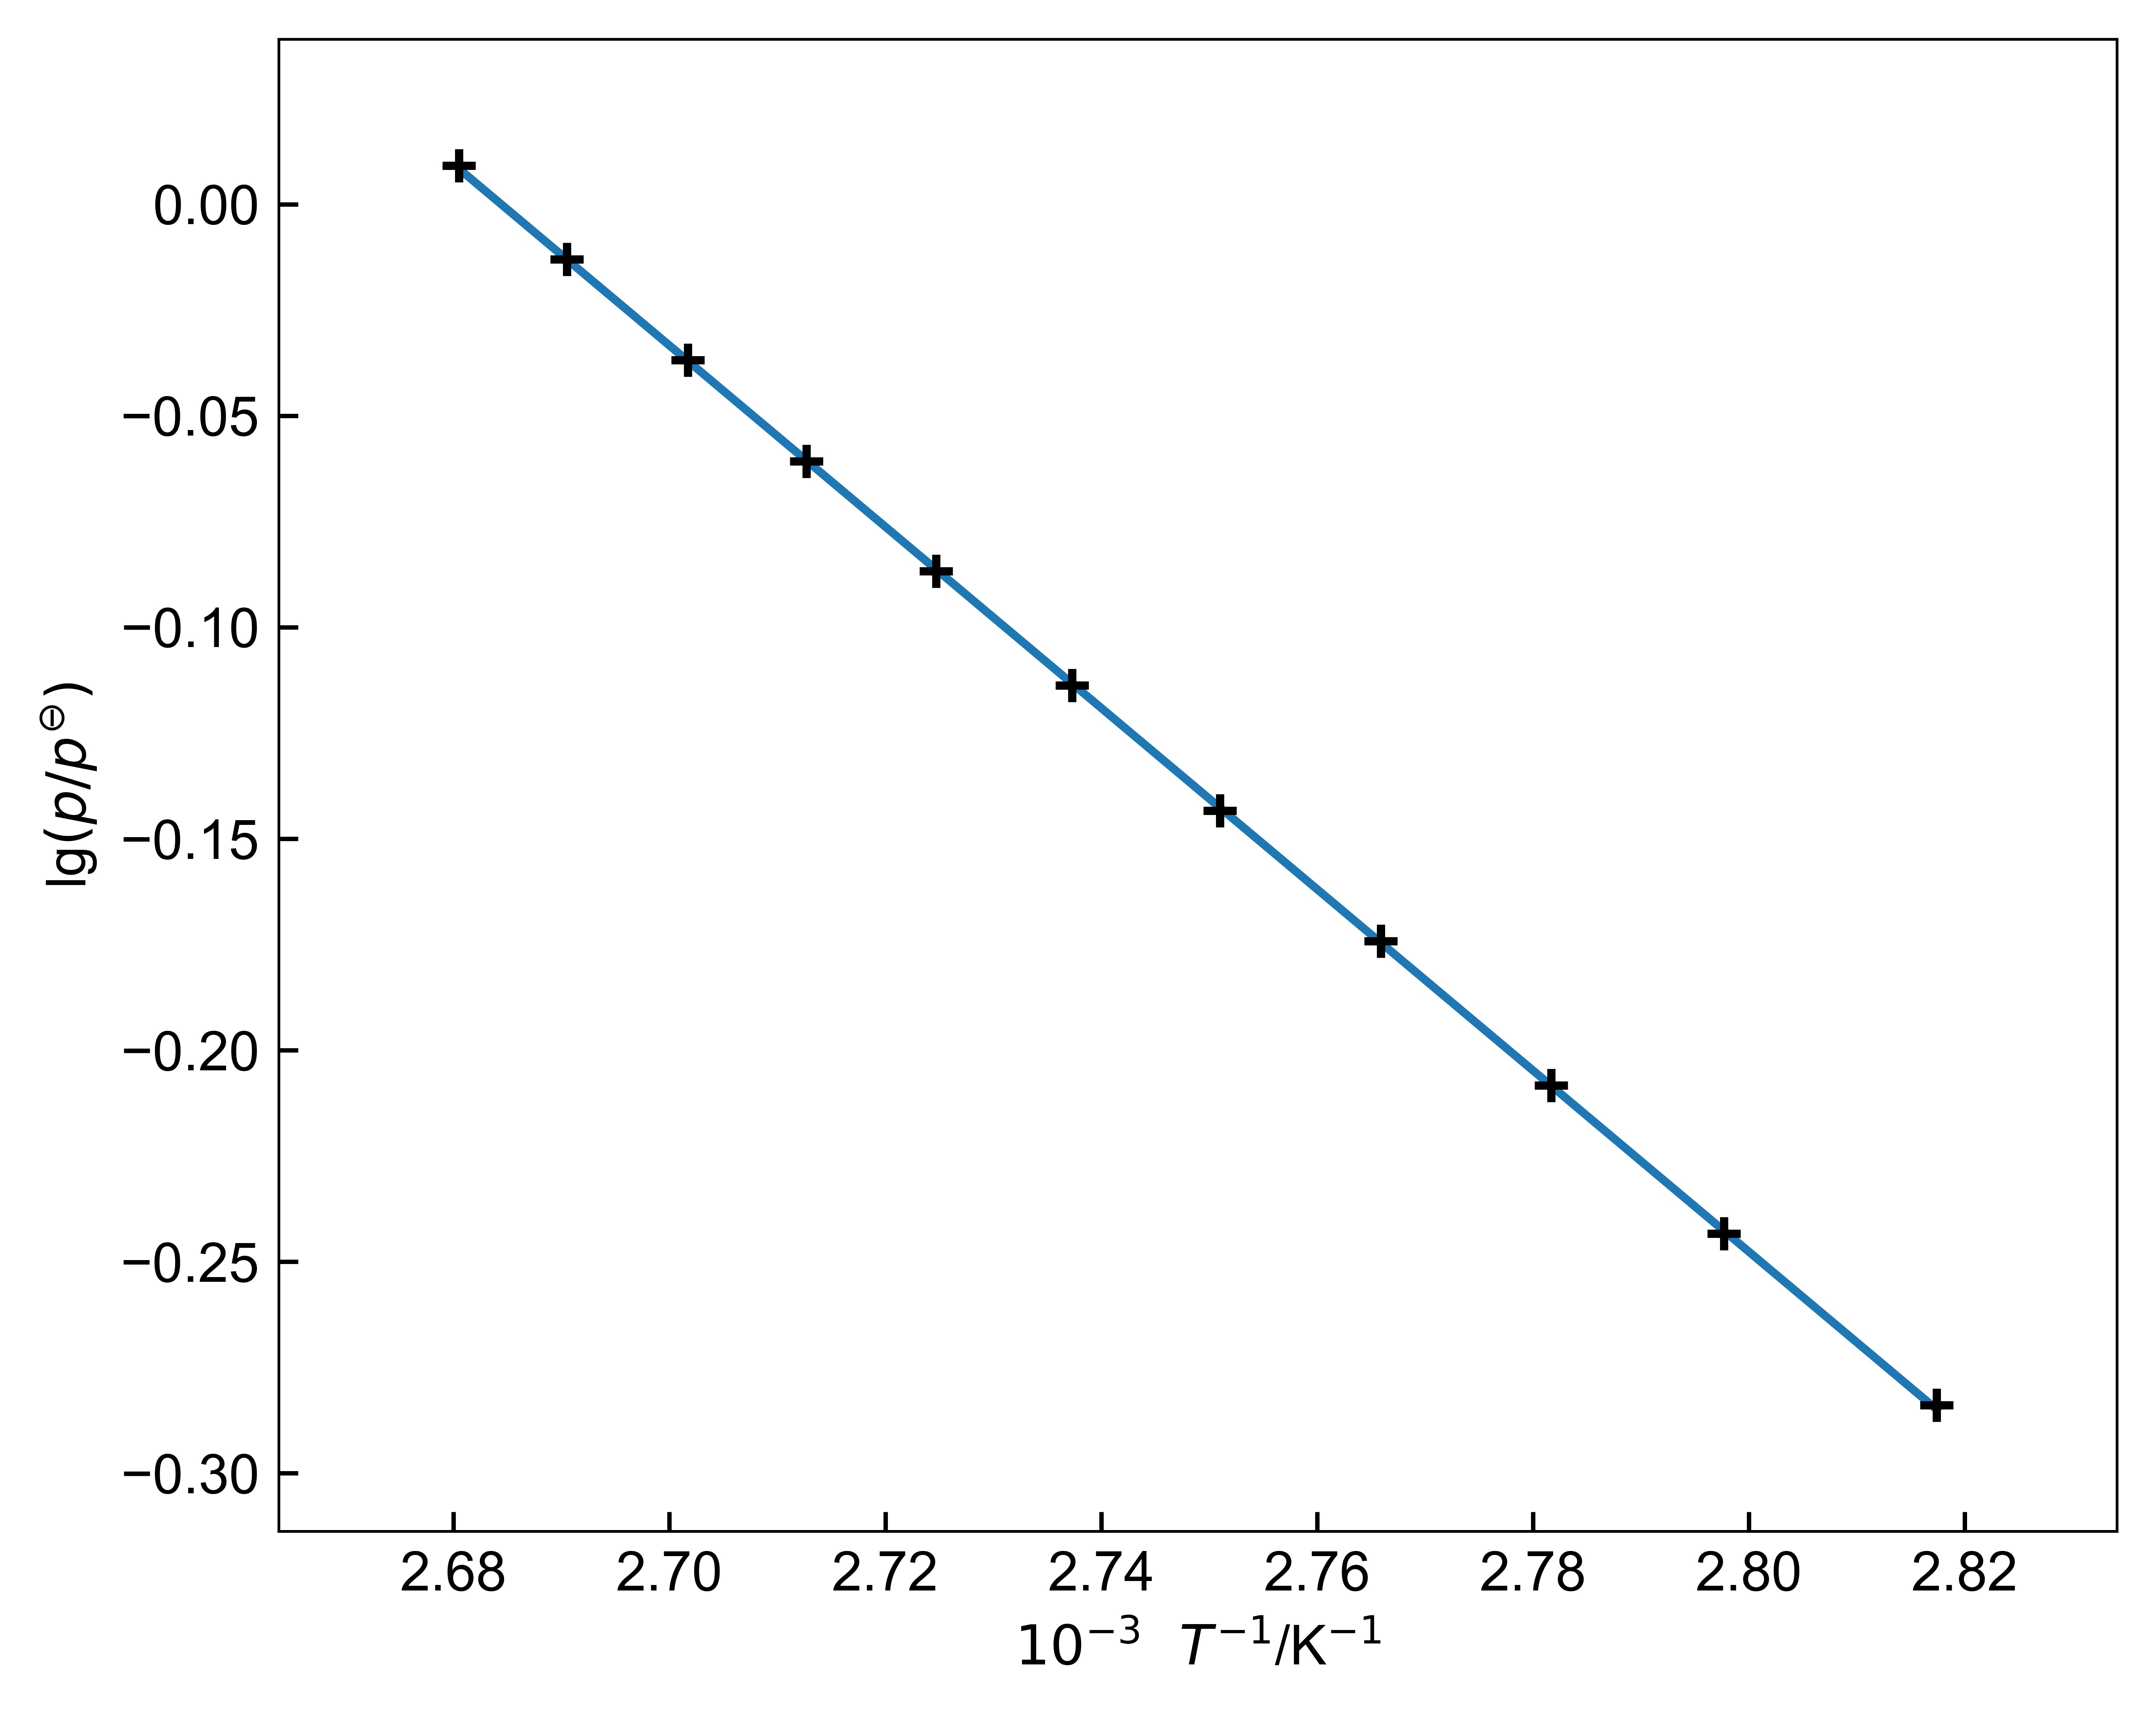
\includegraphics[width=0.6\textwidth]{4.jpg}
	\bicaption{$\rm H_{2}O \ \ $ ${\rm lg}(p/p^{\ominus})$-$T^{-1}$拟合直线}{${\rm lg}(p/p^{\ominus})$-$T^{-1}$ Fitted Curve of $\rm H_{2}O$}
\end{figure}
\par
拟合直线的方程为
$$
{\rm lg}(p/p^{\ominus})=-(2.142\pm 0.004)\times 10^{3} \ \ T^{-1}/{\rm K^{-1}}+(5.75\pm 0.01),\   \  R=-0.99998
$$
$|R|\approx 1$,可见${\rm lg}(p/p^{\ominus})$-$T^{-1}$具有很好的线性关系,与Clausius-Clapeyron方程相符。\par 
根据\textbf{图4}中${\rm lg}(p/p^{\ominus})$-$T^{-1}$拟合直线的方程,代入$p=1\ \ {\rm atm}=101.3\ \ {\rm kPa}$,计算$\rm H_{2}O$的沸点
$$
T=(373\pm 1)\ \ {\rm K}=(100\pm 1)\ \ {\rm ^{\circ}C}  
$$
查阅\textit{CRC Handbook of Chemistry and Physics}\citealp{crc},知$\rm H_{2}O$在$\rm 1\ \ atm$下的沸点$t_{b}=100.0\ \ {\rm ^{\circ}C}$,实验计算结果与参考值相近。\par 
计算$\rm H_{2}O$的平均摩尔气化热$\Delta^{\rm g}_{\rm l}H_{m}$。根据拟合直线斜率大小
$$
A=\frac{\Delta^{\rm g}_{\rm l}H_{m}}{2.303R}
$$
计算
$$
\Delta^{\rm g}_{\rm l}H_{m}=-2.303RA=41.01\ \ {\rm kJ\cdot mol^{-1}}
$$
$\Delta^{\rm g}_{\rm l}H_{m}$的不确定度
$$
\sigma_{\Delta^{\rm g}_{\rm l}H_{m}}=2.303R\sigma_{A}=0.08\ \ {\rm kJ\cdot mol^{-1}}
$$
故$\rm H_{2}O$的平均摩尔气化热
$$
\Delta^{\rm g}_{\rm l}H_{m}=(41.01\pm 0.08)\ \ {\rm kJ\cdot mol^{-1}}
$$
查阅\textit{CRC Handbook of Chemistry and Physics}\citealp{crc},知$\rm H_{2}O$在常压沸点下$\Delta^{\rm g}_{\rm l}H_{m}=40.65\ \ {\rm kJ\cdot mol^{-1}}$,实验计算结果与参考值相当接近。
\par
计算$\rm H_{2}O$的摩尔气化熵$\Delta^{\rm g}_{\rm l}S_{m}$。
根据3.1.2,实验测得$\rm H_{2}O$常压沸点
$$
T_{b}=(373.50\pm 0.01)\ \ {\rm K}
$$
在常压沸点$t_{b}$下,自由能变$\Delta^{\rm g}_{\rm l}G_{m}=0$,故
$$
\Delta^{\rm g}_{\rm l}S_{m}=\frac{\Delta^{\rm g}_{\rm l}H_{m}}{T_{b}}=\frac{41.01\ \ {\rm kJ\cdot mol^{-1}}}{373.50\ \ {\rm K}}=109.8\ \ {\rm J\cdot K^{-1} \cdot mol^{-1}}
$$
$\Delta^{\rm g}_{\rm l}S_{m}$的不确定度
$$
\sigma_{\Delta^{\rm g}_{\rm l}S_{m}}=\frac{1}{T_{b}} \sqrt{\sigma^{2}_{\Delta^{\rm g}_{\rm l}H_{m}}+\frac{\Delta^{\rm g}_{\rm l}H_{m}^{2}}{T_{b}^{2}}\sigma^{2}_{t_{b}}}=0.2\ \ {\rm J\cdot K^{-1}\cdot mol^{-1}}
$$
故$\rm H_{2}O$的摩尔气化熵
$$
\Delta^{\rm g}_{\rm l}S_{m}=(109.8\pm 0.2)\ \ {\rm J\cdot K^{-1} \cdot mol^{-1}}
$$
根据褚鲁统规则,在常压沸点下各正常液体的摩尔气化熵相同,为$\Delta S\approx 88\ \ {\rm J\cdot K^{-1}\cdot mol^{-1}}$。实验得到$\rm H_{2}O$摩尔气化熵的计算结果与褚鲁统规则偏差较大,远大于$88\ \ {\rm J\cdot K^{-1}\cdot mol^{-1}}$。分析可能的原因是液态水中存在大量分子间氢键,在气化过程中需克服氢键相互作用,带来了额外的熵效应,故水的摩尔气化熵明显$>88\ \ {\rm J\cdot K^{-1}\cdot mol^{-1}}$,偏离褚鲁统规则。
 	 \section{讨论与结论}
		\subsection{实验讨论}
 			\subsubsection{静态法测$\rm CCl_{4}$ $\Delta^{\rm g}_{\rm l}H_{m}$的结果评价与误差分析}
本实验的关键是平均摩尔气化热$\Delta^{\rm g}_{\rm l}H_{m}$的准确测定,摩尔气化熵$\Delta^{\rm g}_{\rm l}S_{m}$计算的准确度很大程度地依赖平均摩尔气化热测定的准确度。下面对平均摩尔气化热的测定结果进行定量评价和误差分析。
本实验使用静态法测定$\rm CCl_{4}$的平均摩尔气化热$\Delta^{\rm g}_{\rm l}H_{m}=(30.87\pm 0.02)\ \ {\rm kJ\cdot mol^{-1}}$,对比文献参考值\citealp{crc}$\Delta^{\rm g}_{\rm l}H_{m}=29.82\ \ {\rm kJ\cdot mol^{-1}}$,实验测定值略大于文献参考值,结果的相对误差
$$
\xi=\frac{30.87-29.82}{29.82}\times 100\%=3.52\%
$$
可知测定结果的相对误差在可接受范围内,$\Delta^{\rm g}_{\rm l}H_{m}$测定较为准确。经分析,静态法测$\Delta^{\rm g}_{\rm l}H_{m}$可能的误差来源包括:
\par 
(1)平衡管内空气可能未完全排净,$c$两管液面上方仍存在少量空气,使得$\rm CCl_{4}$的饱和蒸气压与实际压强略有偏差;\par 
(2)实验中温度计测量温度为水浴温度,而实验中温度变化较快,不能保证平衡管与水浴时刻保持热平衡,测得温度与$\rm CCl_{4}$实际温度有一定偏差;\par 
(3)实验中以平衡管$b$、$c$两管液面等高时的压力计示数作为压差值,而实验过程中液面的移动并不匀速,严格上两管液面等高并不能保证两端压强相等,从而为饱和蒸气压$p$的测量引入误差。\par 
\subsubsection{动态法测$\rm H_{2}O$ $\Delta^{\rm g}_{\rm l}H_{m}$的结果评价与误差分析} 
本实验使用动态法测定$\rm H_{2}O$的平均摩尔气化热$\Delta^{\rm g}_{\rm l}H_{m}=(41.01\pm 0.08)\ \ {\rm kJ\cdot mol^{-1}}$,对比文献参考值\citealp{crc}$\Delta^{\rm g}_{\rm l}H_{m}=40.65\ \ {\rm kJ\cdot mol^{-1}}$,实验测定值略大于文献参考值,结果的相对误差
$$
\xi=\frac{41.01-40.65}{40.65}\times 100\%=0.88\%
$$
可知测定结果的相对误差在可接受范围内,$\Delta^{\rm g}_{\rm l}H_{m}$测定相当准确。经分析,动态法测$\Delta^{\rm g}_{\rm l}H_{m}$可能的误差来源包括:
\par 
(1)在实验过程中,观察到烧瓶内液体浑浊,推测在加热回流过程中部分真空脂混溶于去离子水中,一定程度上影响了测得$\rm H_{2}O$的热学性质;\par 
(2)温度计放置位置一定程度上影响测定准确性,若温度计位置在液面以下,测得温度可能为未沸腾部分水的温度,为温度测量引入一定误差。\par
就结果而言,本次实验中动态法结果的相对误差$\xi$小于静态法。



 	 \subsection{实验结论}
本实验使用静态法测$\rm CCl_{4}$不同温度的饱和蒸气压,测得$\rm CCl_{4}$常压沸点$T_{b}=(350.17\pm 0.01)\ \ {\rm K}$;根据实验数据作出$p-T$曲线和${\rm lg}(p/p^{\ominus})$拟合直线,根据拟合直线斜率大小计算$\rm CCl_{4}$的平均摩尔气化热$\Delta^{\rm g}_{\rm l}H_{m}=(30.87\pm 0.02)\ \ {\rm kJ\cdot mol^{-1}}$,摩尔气化熵$\Delta^{\rm g}_{\rm l}S_{m}=(88.16\pm 0.06)\ \ {\rm J\cdot K^{-1}\cdot mol^{-1}}$。各热力学数据计算值与文献参考值相近。\par 
使用动态法测$\rm H_{2}O$不同温度的饱和蒸气压,测得$\rm H_{2}O$常压沸点$T_{b}=(373.50\pm 0.01)\ \ {\rm K}$;根据实验数据作出$p-T$曲线和${\rm lg}(p/p^{\ominus})$拟合直线,根据拟合直线斜率大小计算$\rm H_{2}O$的平均摩尔气化热$\Delta^{\rm g}_{\rm l}H_{m}=(41.01\pm 0.08)\ \ {\rm kJ\cdot mol^{-1}}$,摩尔气化熵$\Delta^{\rm g}_{\rm l}S_{m}=(109.8\pm 0.2)\ \ {\rm J\cdot K^{-1}\cdot mol^{-1}}$。各热力学数据计算值与文献参考值相近。\par 
本实验验证了$\rm CCl_{4}$的摩尔气化熵大致符合褚鲁统规则预测,而$\rm H_{2}O$不符合褚鲁统规则,分析可能原因是$\rm H_{2}O$中分子间氢键的存在使得摩尔气化熵偏离褚鲁统规则。


 

   

\vbox{}

\bibliographystyle{achemso}
\bibliography{a}



\end{document}